% Author: Carles Marin (Claude, Anthropic, as AI research assistant).
% Anomaly- and Tadpole-Compatible Fermion Completion of 6D SU(4) Gauge-Higgs Unification.
% Question-threaded narrative; physics first, exact method in support. Build: pdflatex x2.
\documentclass[11pt,a4paper]{article}
\usepackage[utf8]{inputenc}
\usepackage{amsmath,amssymb,amsthm}
\usepackage{booktabs}
\usepackage[table,dvipsnames]{xcolor}
\usepackage{graphicx}
\usepackage{tikz}
\usetikzlibrary{shapes.geometric,arrows.meta,positioning,fit,backgrounds}
\usepackage{geometry}
\geometry{margin=2.4cm}
\usepackage[colorlinks=true,linkcolor=RoyalBlue,citecolor=BrickRed,urlcolor=RoyalBlue]{hyperref}
\usepackage{caption}
\captionsetup{font=small,labelfont=bf}
\newtheorem{proposition}{Proposition}
\newtheorem{theorem}{Theorem}
\newcommand{\ZZ}{\mathbb{Z}}
\newcommand{\Tr}{\mathrm{Tr}}
\definecolor{okgreen}{RGB}{0,140,54}
\definecolor{hdrblue}{RGB}{31,78,121}
\definecolor{softgrey}{RGB}{238,242,247}

\title{\textbf{Anomaly- and Tadpole-Compatible Fermion Completion of\\
Six-Dimensional $SU(4)$ Gauge--Higgs Unification}\\[4pt]
\large\textnormal{An exact consistency analysis --- machine-checked and independently verified --- and the boundary-mass filter}}
\author{Carles Mar\'in\thanks{Independent researcher, \texttt{karlesmarin@gmail.com}.
The exact computations were carried out and cross-checked with Claude (Anthropic) as
an AI research assistant against a common machine-verifiable ground truth (Lean,
exact algebra); all results are reproducible from the ancillary
scripts and the Lean certificate.}}
\date{\today\\[2pt]\small DOI: \href{https://doi.org/10.5281/zenodo.21432626}{10.5281/zenodo.21432626}}

\begin{document}
\maketitle

\begin{abstract}
\noindent
In gauge--Higgs unification the cancellation of gauge anomalies is necessary, but is
it sufficient for a viable fermion sector? On an orbifold the answer involves genuinely
\emph{local} data --- anomalies and tadpoles bound to the fixed points --- that a bulk
count misses. We make the question concrete for a colored quark block embedded in the
dimension-$60$ representation $(3,\mathbf{60})$ of $SU(4)$ on $T^2/\mathbb{Z}_2$, built
over the two-Higgs-doublet gauge sector of Akamatsu, Hirose, Maru and Nago
(AHMN)~\cite{AHMN}; the fermion embedding is our own. We fix the unique unbroken
hypercharge that reproduces the Standard-Model quark charges, and organize every
consistency requirement into a reproducible hierarchy of exact conditions: the
irreducible six-dimensional and four-dimensional zero-mode anomalies, the localized
non-Abelian cubic residues (certified axiom-free in the Lean~4 proof assistant), the
localized tadpole, the global $SU(2)$ (Witten) constraint, and the boundary-mass
matching of exotic zero modes. We then exhibit --- and independently verify in exact
rational arithmetic --- a $45$-multiplet completion that cancels the eight anomaly
coefficients and the localized tadpole together, with integral local cubic residues,
so that here anomaly freedom and the tadpole condition are \emph{compatible}. This is not
accidental. That the two constraints are \emph{independent} was observed long ago by
Scrucca, Serone, Silvestrini and Wulzer~\cite{SSSW}, who left the construction of an
anomaly-free spectrum with globally vanishing tadpole as an open problem; we make the
independence exact and, beyond it, prove that anomaly-neutral matter realizes \emph{any}
tadpole, so \emph{every} anomaly-free completion of the block is tadpole-compatible ---
settling that open requirement as a structural guarantee, with the exact rank-and-cone
test released as a reusable tool. The
decisive remaining test, whether the exotics can be given mass without lifting the
Standard-Model quarks, is cast as an exact bipartite-matching gate and left open
pending the full brane spectrum. Every step is a finite exact computation; the general
bounded search is hard and stays open, but the results we report are certificates, not
estimates.
\end{abstract}

% ===================================================================
\section{Gauge--Higgs unification and the subtlety of orbifolds}\label{sec:intro}
If a six-dimensional fermion content cancels every gauge anomaly, is the resulting
four-dimensional theory automatically healthy? The question is as old as the idea that
the Higgs boson need not be an elementary scalar. In 1979 Manton and Fairlie observed
that, with extra dimensions, the internal components of a higher-dimensional gauge
field transform as four-dimensional scalars, so a Higgs doublet can arise as a
low-energy mode of the gauge connection itself~\cite{Manton,Fairlie}. Hosotani turned
this kinematic remark into a dynamical mechanism: the Wilson-line phases wrapping a
compact dimension are physical, and their expectation values break the gauge
symmetry~\cite{Hosotani}. In this \emph{gauge--Higgs unification} (GHU) the Higgs
potential vanishes at tree level and is generated radiatively, so the electroweak scale
is finite and calculable --- the original motivation, and still the appeal: a Higgs
mass protected from ultraviolet sensitivity by higher-dimensional gauge invariance.

Two further ingredients make such a picture realistic: chiral fermions, and a breaking
of the unified group to the Standard Model. Orbifold compactifications supply both.
Kawamura's construction breaks a grand-unified $SU(5)$ to the Standard Model by
boundary conditions on $S^1/(\mathbb{Z}_2\times\mathbb{Z}_2')$, projecting out the
dangerous colored Higgs while keeping the doublet --- and doing so without a
symmetry-breaking potential~\cite{KawamuraGUT}. The economy carries a subtle price.
An orbifold is not a manifold; its fixed points are singular loci that host their own,
\emph{local}, physics. Anomalies need not cancel point by point in the naive way.
Arkani-Hamed, Cohen and Georgi showed that the higher-dimensional anomaly localizes on
the fixed planes, so that four-dimensional anomaly cancellation in the low-energy
spectrum controls the consistency of the whole construction~\cite{ACG}; von Gersdorff
and Quir\'os developed the localized-anomaly formalism in five and six dimensions and
its cancellation by inflow and by brane fields~\cite{GdVQ,GdV6D}. A second local effect
is equally consequential: radiatively generated tadpoles for the internal gauge field
(the would-be Higgs) at the fixed points, which feed directly into the Higgs mass and
can spoil the calculability that motivated the whole framework. Biggio and Quir\'os
gave the symmetry criteria for when such tadpoles appear, and showed that in six
dimensions on $T^2/\mathbb{Z}_2$ they arise for fermions in essentially arbitrary
representations~\cite{BiggioQ}. Scrucca, Serone, Silvestrini and Wulzer sharpened the
tension into a question. A six-dimensional fermion contributes to the tadpole with a sign
fixed by its representation but \emph{independent} of its chirality; so, they observed,
the vanishing-tadpole and anomaly-cancellation requirements are ``in general independent
constraints'' --- cancelling the anomalies buys nothing for the tadpole, and cancelling
the tadpole buys nothing for the anomalies. They then named the missing piece plainly: a
realistic model must rest on ``an anomaly-free fermion spectrum with a globally vanishing
tadpole''~\cite{SSSW}, and left that as an open problem, with a doubtful note on whether
it could be met at all. That question, posed in 2003, is the one this paper takes up. A
bulk anomaly count, in short, is necessary but not sufficient --- which is the question
above, made concrete.

Our arena is the recent six-dimensional $SU(4)$ model of AHMN~\cite{AHMN}, in which
\emph{two} Higgs doublets appear as zero modes of the extra-dimensional gauge field on
$T^2/\mathbb{Z}_2$. AHMN specify the gauge and Higgs sectors; the fermion content that
would reproduce the Standard-Model quarks is not part of their construction, and it is
there that we work. We embed a colored quark block in the dimension-$60$ representation
$(3,\mathbf{60})$ of $SU(4)$ --- \emph{our} construction, not theirs --- and ask
whether it can be completed into a consistent, and ultimately viable, fermion sector.
Answering that means passing the full hierarchy of conditions above; our contribution
is to impose every one of them \emph{exactly}, as a machine-checkable certificate
rather than a case-by-case argument, and to report honestly where the concrete model
stands.

\paragraph{Scope and relation to prior work.} The general ingredients are established.
The mechanism of gauge--Higgs unification in orbifold models, and systematic
classifications of anomaly-free orbifold-GUT and GHU matter, are well
developed~\cite{SSSW,Kawamura,aGUT,SU6GHGUT}; localized anomalies~\cite{ACG,GdVQ,GdV6D} and
localized tadpoles~\cite{BiggioQ} are textbook consistency conditions. We claim no new
general physics. What is new here is ours on three counts: (i) the specific
$SU(4)/T^2\mathbb{Z}_2$ crossing --- integer fermion completion subject to localized
anomalies, tadpoles and exotic matching, all at once; (ii) the \emph{exact, reproducible}
protocol in which every condition is recomputed exactly and independently verified, with
the localized-anomaly fragment machine-checked in Lean~4; and (iii) the structural result
that this study yields --- our Existence theorem (\S\ref{sec:existence},
Theorem~\ref{thm:existence}): that the localized tadpole \emph{never obstructs} an
anomaly-free completion, which settles as a structural guarantee the
anomaly-free-spectrum-with-vanishing-tadpole problem left open by
Scrucca et al.~\cite{SSSW}. That the two constraints are \emph{independent} was already
their observation; our new step is the reachability result that turns independence into a
no-obstruction guarantee --- made exact, machine-checked, and packaged as a reusable tool.
The linear-algebra ingredients (rank tests, Farkas duality) are standard; what is ours is
the reachability theorem, its certificates, and their application here. The physical
verdict on viability is not yet closed, and we say so throughout.

\begin{figure}[t]
\centering
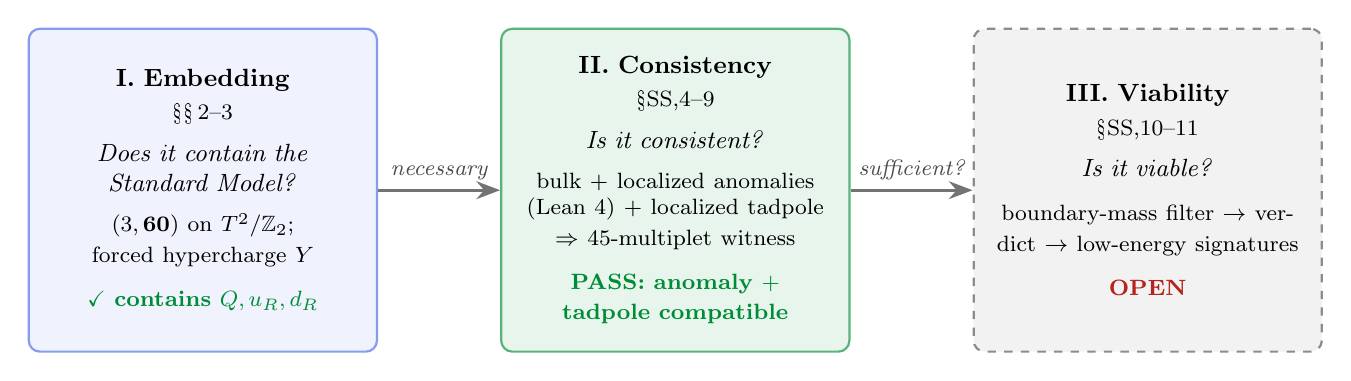
\begin{tikzpicture}[font=\small,
  act/.style={rounded corners,draw,thick,text width=4.0cm,align=center,inner sep=6pt,minimum height=4.1cm,anchor=north},
  arr/.style={-{Stealth[length=3mm]},very thick,black!55}]
\node[act,fill=RoyalBlue!8,draw=RoyalBlue!65] (a1) at (0,0)
 {\textbf{I.\ Embedding}\\[1pt]{\footnotesize\S\S\,2--3}\\[4pt]
  \textit{Does it contain the}\\\textit{Standard Model?}\\[5pt]
  {\footnotesize $(3,\mathbf{60})$ on $T^2/\mathbb{Z}_2$;\\ forced hypercharge $Y$}\\[5pt]
  {\footnotesize\color{okgreen}\textbf{$\checkmark$ contains $Q,u_R,d_R$}}};
\node[act,fill=okgreen!9,draw=okgreen!65] (a2) at (6.0,0)
 {\textbf{II.\ Consistency}\\[1pt]{\footnotesize\S\SS,4--9}\\[4pt]
  \textit{Is it consistent?}\\[5pt]
  {\footnotesize bulk $+$ localized anomalies (Lean~4) $+$ localized tadpole\\$\Rightarrow$ $45$-multiplet witness}\\[5pt]
  {\footnotesize\color{okgreen}\textbf{PASS: anomaly $+$ tadpole compatible}}};
\node[act,fill=black!5,draw=black!45,dashed] (a3) at (12.0,0)
 {\textbf{III.\ Viability}\\[1pt]{\footnotesize\S\SS,10--11}\\[4pt]
  \textit{Is it viable?}\\[5pt]
  {\footnotesize boundary-mass filter $\rightarrow$ verdict $\rightarrow$ low-energy signatures}\\[5pt]
  {\footnotesize\color{BrickRed}\textbf{OPEN}}};
\draw[arr] (a1.east) -- node[above,font=\footnotesize\itshape,black!70]{necessary} (a2.west);
\draw[arr] (a2.east) -- node[above,font=\footnotesize\itshape,black!70]{sufficient?} (a3.west);
\end{tikzpicture}
\caption{The journey of this paper. We ask three questions in turn --- does the
representation contain the Standard-Model quarks, is the resulting theory consistent, and
is it physically viable --- each a stricter test than the last. The embedding and the
consistency conditions are settled exactly (the localized anomalies machine-checked in
Lean); the viability verdict, gated by the boundary-mass filter, is left open.}
\label{fig:roadmap}
\end{figure}

\begin{table}[t]
\centering\small
\newcommand{\ye}{\textcolor{okgreen}{\checkmark}}
\newcommand{\no}{\textcolor{BrickRed}{\ensuremath{\times}}}
\resizebox{\textwidth}{!}{%
\begin{tabular}{lccccc}
\toprule
\rowcolor{hdrblue}
\textcolor{white}{Treatment of the fermion sector} & \textcolor{white}{Bulk} &
\textcolor{white}{Localized} & \textcolor{white}{Tadpole} &
\textcolor{white}{Exact} & \textcolor{white}{Lean}\\
\midrule
AHMN gauge--Higgs construction~\cite{AHMN}        & \ye & \no & \no & \no & \no\\
Orbifold-GUT/GHU classifications~\cite{Kawamura,aGUT,SU6GHGUT} & \ye & \ye & \no & \no & \no\\
\rowcolor{softgrey}\textbf{This work} & \ye & \ye & \ye & \ye & \ye\\
\bottomrule
\end{tabular}}
\caption{What each analysis establishes for the fermion sector of this class of
six-dimensional orbifold models. AHMN~\cite{AHMN} supply the gauge and two-Higgs sector
we build on; systematic classifications treat bulk and localized anomalies; the present
work adds the localized tadpole, an exact integer completion, and a Lean-checked fragment,
imposing all of them together. Checkmarks indicate that the condition is treated for a
concrete quark completion, not merely in principle.}
\label{tab:compare}
\end{table}

% ===================================================================
\section{Gauge--Higgs unification on \texorpdfstring{$T^2/\mathbb{Z}_2$}{T2/Z2}}\label{sec:orbifold}
We work on $M^4\times T^2/\mathbb{Z}_2$. The torus is coordinatized by
$(y_5,y_6)$ with identifications $y_i\sim y_i+2\pi R_i$; the $\mathbb{Z}_2$ acts by
$(y_5,y_6)\to(-y_5,-y_6)$ and leaves four fixed points. The six-dimensional gauge field
decomposes into a four-dimensional vector $A_\mu$ and two internal scalars $A_5,A_6$;
under the orbifold projection the surviving zero modes of $A_{5,6}$ are the Higgs
fields. In the AHMN $SU(4)$ model the projection at the four fixed points is governed
by two commuting parities,
\begin{equation}
P_0=P_1=\mathrm{diag}(+,+,+,-),\qquad P_2=P_3=\mathrm{diag}(+,+,-,-),
\end{equation}
so the four fixed points fall into two classes with distinct unbroken local groups,
\begin{equation}
f=0,1:\ SU(3)_C\times SU(3)_{123}\times U(1)_{15},\qquad
f=2,3:\ SU(3)_C\times SU(2)_{12}\times SU(2)_{34}\times U(1)_P .
\end{equation}
The four-dimensional gauge group left unbroken everywhere is the intersection
$SU(3)_C\times SU(2)_L\times U(1)_Y$ (times a residual $U(1)$), and two Higgs doublets
arise from the $A_5,A_6$ zero modes~\cite{AHMN}. The tree-level Higgs potential is the
internal field strength, $V_{\rm tree}\propto \Tr[A_5,A_6]^2$, and vanishes for flat
(commuting) configurations. This makes the Higgs elusive by construction: it is a
Wilson line, a holonomy phase detectable only by transporting a field once around the
compact dimension, so in what sense is it a local field with a mass at all? The answer
is the mechanism's whole point. The physical potential is generated radiatively, of
Coleman--Weinberg type~\cite{ColemanWeinberg} in the Wilson-line phase; because the
would-be Higgs is a component of a gauge field, higher-dimensional gauge invariance
forbids a local mass counterterm and the potential is finite and calculable, the
property that made GHU attractive in the first place~\cite{Hosotani}. The Higgs's very
non-locality is thus its protection --- there is no local operator to renormalize its
mass --- and a field with no tree-level potential nonetheless chooses a vacuum, born
entirely of the quantum response of the tower of modes to the Wilson-line phase. It is exactly this
calculability that a localized tadpole endangers: a fixed-point term linear in the
internal field feeds directly into the Higgs mass and is \emph{not} protected, so
demanding its absence is on the same footing as anomaly freedom, not a cosmetic
addition.

Throughout we label an $SU(4)$ weight by the Young entries $n_1\ge n_2\ge n_3\ge n_4$
of the corresponding tableau; the useful internal charges are
$q_8=n_1+n_2-2n_3$, $q_{15}=n_1+n_2+n_3-3n_4$ and $q_P=n_1+n_2-n_3-n_4$, and the two
$\mathbb{Z}_2$ parities of a weight are $p_0=(-1)^{n_4}$ and $p_2=(-1)^{n_3+n_4}$.
These are the data every exact condition below is built from.

% ===================================================================
\section{The \texorpdfstring{$(3,\mathbf{60})$}{(3,60)} quark block and its hypercharge}\label{sec:hypercharge}
Before any consistency condition one must ask whether the chosen representation even
contains the Standard-Model quarks, and under which unbroken hypercharge. We embed the
quarks in the colored block $(3,\mathbf{60})$, the color triplet times the
dimension-$60$ irrep $(0,2,1)$ of $SU(4)$. It contains $Q$, $u_R$, $d_R$ under a
hypercharge that is essentially forced: among the internal mixings it is the unique
combination preserving $\sin^2\theta_W=\tfrac14$ at tree level,
\begin{equation}
\boxed{\;Y=\frac{-7\,q_8+4\,q_{15}}{18}\;},\qquad Q_{\rm em}=T_3+Y .
\label{eq:Y}
\end{equation}
Equation~\eqref{eq:Y} reproduces the Standard-Model quark charges exactly
(Table~\ref{tab:smcontent}); everything else in the multiplet is an exotic that a
consistent theory must ultimately remove. Two features already visible will drive the
rest of the analysis. First, $Q_L$ appears with multiplicity two: one combination is
the physical doublet, the other an exotic of identical gauge charges --- so lifting the
exotic doublet without lifting $Q_L$ is a nontrivial, rank-level question. Second, the
exotic zero modes are left-handed doublets and a quartet together with right-handed
singlets and triplets: their $SU(2)_L$ representations do not match across chirality,
so they cannot pair among themselves and require brane partners.
\emph{Established here:} the $(3,\mathbf{60})$ does contain the three Standard-Model
quark multiplets under a single, essentially forced hypercharge. \emph{Left open:} the
remaining exotic zero modes it also carries, which the consistency gates below must
remove without touching $Q,u_R,d_R$.

The choice of $(3,\mathbf{60})$ is one of economy, not taste. Scanning \emph{all}
$SU(4)$ irreps of dimension $\le 63$, only two have $T^2/\mathbb{Z}_2$ zero modes that
contain a complete Standard-Model quark generation ($Q_L,u_R,d_R$ as color triplets)
under a single unbroken hypercharge: the $\mathbf{60}=(0,2,1)$ used here and its
conjugate $(1,2,0)$, \emph{both} of dimension $60$. No smaller colored $SU(4)$ block
does. In that precise, checked sense $(3,\mathbf{60})$ is the minimal representation
that can host the quarks at all --- which is why it, and not some smaller multiplet, is
the natural place to test whether a consistent completion exists. \emph{Why} only these
representations, and why so few, is turned from this scanned fact into an exact closed
criterion in the companion Part~II~\cite{PartII}.

\begin{table}[t]
\centering
\rowcolors{2}{softgrey}{white}
\begin{tabular}{lccccl}
\toprule
\rowcolor{hdrblue}
\textcolor{white}{Field} & \textcolor{white}{$SU(2)_L$} & \textcolor{white}{$(q_8,q_{15})$}
& \textcolor{white}{$Y$} & \textcolor{white}{chirality} & \textcolor{white}{status}\\
\midrule
$Q_L$   & $\mathbf{2}$ & $(-1,-1)$ & $1/6$  & L & \textcolor{okgreen}{\textbf{SM target}}\\
$u_R$   & $\mathbf{1}$ & $(0,3)$   & $2/3$  & R & \textcolor{okgreen}{\textbf{SM target}}\\
$d_R$   & $\mathbf{1}$ & $(-2,-5)$ & $-1/3$ & R & \textcolor{okgreen}{\textbf{SM target}}\\
\midrule
\multicolumn{6}{l}{\emph{exotic zero modes}: LH doublets/quartet, RH singlets/triplets --- to be lifted}\\
\bottomrule
\end{tabular}
\caption{Standard-Model quark content of $(3,\mathbf{60})$ under the hypercharge
\eqref{eq:Y}, verified exactly. $Q_L$ occurs with multiplicity two --- one physical,
one exotic --- a fact that returns in \S\ref{sec:n7}.}
\label{tab:smcontent}
\end{table}

% ===================================================================
\section{Bulk anomalies and the reducibility of the color quartic}\label{sec:bulkanom}
Which part of a gauge anomaly is an absolute obstruction, and which part can instead be
shifted into a reducible Green--Schwarz sector? That distinction organizes what a
completion must do. The first requirements are the standard ones: the irreducible
six-dimensional gauge and gravitational anomalies, and the four-dimensional anomalies of
the surviving zero modes. For $(3,\mathbf{60})$ with $\eta=(+,+)$ the eight coefficients
are, exactly,
\begin{equation}
\resizebox{\textwidth}{!}{$\displaystyle
\boxed{\;\big[SU(3)_C^4,\ SU(4)^4,\ \mathrm{grav}_6,\ SU3^3,\ SU3^2Y,\ SU2_L^2Y,\ Y^3,\
\mathrm{grav}^2Y\big]=\Big[60,\,-579,\,180,\,-3,\,\tfrac{17}{6},\,\tfrac{23}{2},\,\tfrac{2293}{18},\,17\Big]\;}$},
\end{equation}
where the hypercharge is the physical one of Eq.~\eqref{eq:Y} throughout (the four
$Y$-dependent entries scale with that normalization). A subtlety controls what a
completion must do with these. The six-dimensional anomaly
polynomial factorizes as
\begin{equation}
\Tr_{(3,\mathbf{60})}F^4=-579\,\Tr_4 F_4^4+30\,C^2+426\,CX+864\,X^2,
\qquad C=\Tr_3 F_C^2,\ X=\Tr_4 F_4^2,
\end{equation}
and only the primitive quartic $SU(4)^4$ coefficient $-579$ is irreducible; $SU(3)$ has
no primitive quartic Casimir, so $\Tr_3 F_C^4=\tfrac12 C^2$ and the ``$SU(3)_C^4$''
piece is a reducible $(\Tr F_C^2)^2$. The reducible gauge quadratic form
$\left(\begin{smallmatrix}30&213\\213&864\end{smallmatrix}\right)$ has rank $2$. This is
where the Green--Schwarz mechanism~\cite{GreenSchwarz} would ordinarily enter: a
two-form field $B$ with coupling $B\wedge\Tr F^2$ cancels an anomaly precisely when the
anomaly polynomial \emph{factorizes} as a product of two four-forms, i.e.\ when the
quadratic form is rank one. In six dimensions this generalizes to several tensor
multiplets, each contributing one rank-one factor~\cite{Sagnotti}, so a rank-two form
needs at least two tensors and an explicit factorization. In the published gauge/BLKT
setup of AHMN there is no such two-form, so the reducible pieces are imposed as
fermionic equations; a multi-tensor branch would have to declare its tensor content and
exhibit the factorization. Reducibility is a property of the color factor alone: it
means the $SU(3)_C^4$ piece \emph{could} be absorbed by a Green--Schwarz two-form, but
it leaves the primitive $SU(4)^4$ index $-579$ untouched. That one has no such escape ---
there is no tensor coupling that factorizes a genuine quartic Casimir --- so it is an
absolute obstruction that the fermion content must cancel outright. Either way the safe, model-independent requirement is to
cancel all eight coefficients on the added fermions, which is what we impose.
\emph{Established:} the eight coefficients are exact, and the color quartic is reducible
so it needs no primitive-quartic tensor. \emph{Left open at this stage:} whether any
spectrum can zero all eight together with the localized data --- the subject of the
gates that follow.

% ===================================================================
\section{Localized anomalies certified in Lean}\label{sec:localized}
Here a puzzle sharpens: how can a purely topological quantity, blind to the Wilson-line
vacuum, nonetheless constrain the very spectrum that does feel it? Beyond the bulk, the
fixed points carry irreducible \emph{local} anomalies. At each
$f=0,1$ point the pure non-Abelian cubic residues of $(3,\mathbf{60})$ are, exactly,
\begin{equation}
\big[\,SU(3)_C^3,\ SU(3)_{123}^3\,\big]_{f=0,1}=\Big[-\tfrac32,\,-\tfrac34\Big].
\end{equation}
The mechanism behind ``removal'' is anomaly inflow: a fixed point behaves like a defect,
and the anomaly of the fermions living on it is cancelled by a current flowing in from
the bulk, in the manner Callan and Harvey identified for zero modes on strings and
domain walls~\cite{CallanHarvey}. Following von Gersdorff~\cite{GdV6D}, fractional
residues are a diagnostic of an \emph{incomplete} bulk spectrum: only once the
irreducible bulk anomaly is cancelled do the local residues become integral, and only
then can inflow plus brane-localized Weyl fermions remove them. A completion must therefore make these residues integers --- a congruence,
not an equality. Two remarks fix the physics. First, the pure non-Abelian cubics carry
no $U(1)$ charge, so they are independent of the Wilson line (the Higgs vacuum): the
brane content they demand is fixed before electroweak breaking, whereas the mixed
$C^2U(1)$ channel does move with the Higgs. Second, because these are finite exact
statements about rational numbers, we can certify them by machine. The file
\texttt{R60LocalizedAnomaly.lean} proves, \emph{axiom-free and \texttt{sorry}-free} in
the Lean~4 kernel, the exact integer numerators underlying the residues ($-6$ and $6$,
the rationals following by the trivial normalizations $\tfrac14$, $-\tfrac18$), the
dimension count, and that the mixed channel depends on the Wilson line while the pure
cubics do not. To our knowledge this is the first fragment of an orbifold-GUT
consistency analysis checked in a proof assistant.
\emph{Established, and machine-checked:} the local cubic residues are exactly
$[-\tfrac32,-\tfrac34]$ and become integral only for a completed bulk. \emph{Left open:}
the specific brane fermions that carry the compensating inflow, which the boundary
spectrum fixes.

% ===================================================================
\section{The localized tadpole and the exact hierarchy}\label{sec:tadpole}
The last local condition before matching is the tadpole. A single bulk Weyl fermion
induces, at one loop, a localized tadpole for the internal gauge field with group
factor $\Theta_{01}\propto\eta_0\,\Tr_R(P_0 T_{15})$ at $f=0,1$ and
$\Theta_{23}\propto\eta_2\,\Tr_R(P_2 T_P)$ at $f=2,3$~\cite{BiggioQ}. For the base block
$(3,\mathbf{60})$ we find, exactly, $\Theta_{\rm base}=(126,-36)$: the isolated block
fails the tadpole gate, and a consistent completion must cancel it. Crucially the
tadpole is independent of the six-dimensional chirality, so a naive fix by adding
vector-like pairs \emph{doubles} rather than cancels it; the cancellation is a genuine
constraint on chiral content, coupled to the anomalies.
\emph{Established:} the isolated block fails the tadpole gate, $\Theta_{\rm
base}=(126,-36)\neq0$. \emph{The open question} --- whether a single completion can
cancel it \emph{together with} all the anomalies --- is settled affirmatively in
\S\ref{sec:witness}.

Table~\ref{tab:gates} collects the full hierarchy. Gates 1--5 are linear or congruence
conditions on the added multiplets; gate~6 is a rank/matching condition. Figure~\ref{fig:funnel}
shows their logic: the $(3,\mathbf{60})$ passes gates 1--4 exactly (gate~3 in Lean),
while the global $SU(2)$ and the boundary-mass matching remain to be applied.

\begin{table}[t]
\centering\footnotesize
\begin{tabular}{clcl}
\toprule
\rowcolor{hdrblue}
\textcolor{white}{\#} & \textcolor{white}{Condition} & \textcolor{white}{Type} & \textcolor{white}{Certificate}\\
\midrule
\rowcolor{softgrey}
1 & Bulk 6D irreducible $SU(4)^4$, $\mathrm{grav}_6$ & equality & exact integer\\
2 & 4D zero-mode anomalies ($SU3^3,SU3^2Y,SU2^2Y,Y^3,\mathrm{grav}^2Y$) & equality & exact rational\\
\rowcolor{softgrey}
3 & Localized cubics $[SU3_C^3,SU3_{123}^3]$ integrality & congruence & \textbf{\color{okgreen}Lean 4}\\
4 & Localized tadpole $\Theta=(\Theta_{01},\Theta_{23})=0$ & equality & exact integer\\
\rowcolor{softgrey}
5 & Global $SU(2)$ (Witten) parity & mod 2 & exact\\
6 & Boundary-mass matching (protecting $Q,u,d$) & rank/matching & exact bipartite\\
\bottomrule
\end{tabular}
\caption{The exact consistency hierarchy for a fermion completion. Gate 3 is
machine-checked in Lean; the rest are exact Sage / OR-Tools computations.}
\label{tab:gates}
\end{table}

\begin{figure}[t]
\centering
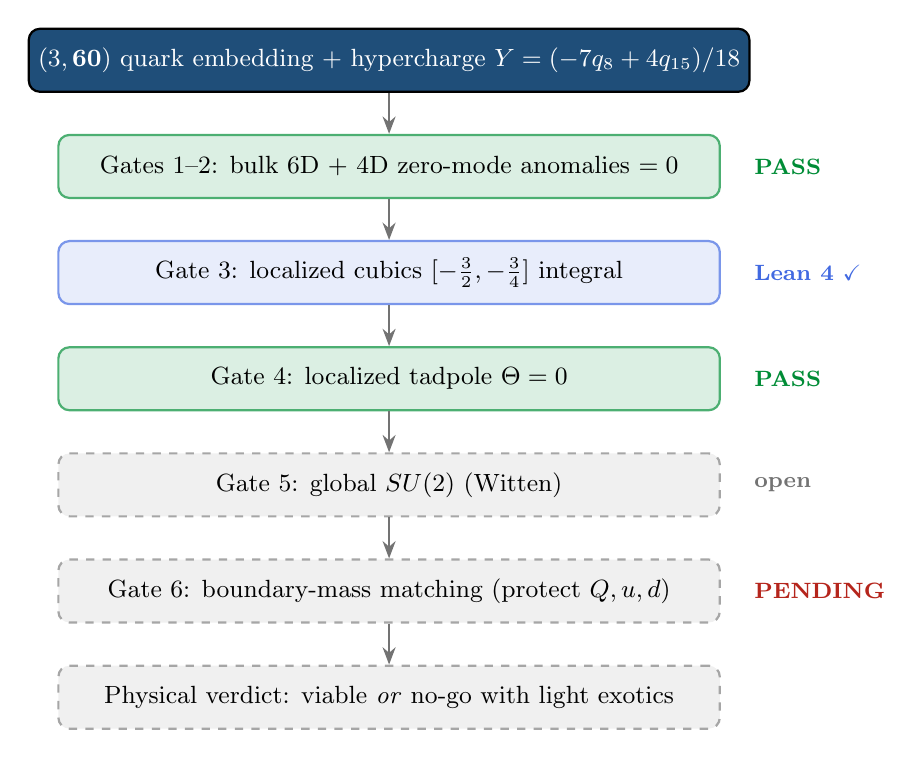
\begin{tikzpicture}[
  node distance=5.2mm,
  gate/.style={rounded corners,draw,thick,minimum width=8.4cm,minimum height=8mm,align=center,font=\small},
  pass/.style={gate,fill=okgreen!14,draw=okgreen!70},
  lean/.style={gate,fill=RoyalBlue!12,draw=RoyalBlue!70},
  open/.style={gate,fill=black!6,draw=black!35,dashed},
  tag/.style={font=\footnotesize\bfseries,anchor=west},
  arr/.style={-{Stealth[length=2.2mm]},thick,black!55}]
\node[gate,fill=hdrblue,text=white] (top) {$(3,\mathbf{60})$ quark embedding $+$ hypercharge $Y=(-7q_8+4q_{15})/18$};
\node[pass,below=of top] (g12) {Gates 1--2: bulk 6D $+$ 4D zero-mode anomalies $=0$};
\node[lean,below=of g12] (g3) {Gate 3: localized cubics $[-\tfrac32,-\tfrac34]$ integral};
\node[pass,below=of g3] (g4) {Gate 4: localized tadpole $\Theta=0$};
\node[open,below=of g4] (g5) {Gate 5: global $SU(2)$ (Witten)};
\node[open,below=of g5] (g6) {Gate 6: boundary-mass matching (protect $Q,u,d$)};
\node[gate,fill=black!6,draw=black!35,dashed,below=of g6] (out) {Physical verdict: viable \emph{or} no-go with light exotics};
\foreach \a/\b in {top/g12,g12/g3,g3/g4,g4/g5,g5/g6,g6/out} \draw[arr] (\a)--(\b);
\node[tag,text=okgreen,right=3mm of g12] {PASS};
\node[tag,text=RoyalBlue,right=3mm of g3] {Lean 4 $\checkmark$};
\node[tag,text=okgreen,right=3mm of g4] {PASS};
\node[tag,text=black!55,right=3mm of g5] {open};
\node[tag,text=BrickRed,right=3mm of g6] {PENDING};
\end{tikzpicture}
\caption{The exact consistency funnel. The $45$-multiplet completion of
\S\ref{sec:witness} passes gates 1--4 exactly, gate~3 machine-checked in Lean; the
global $SU(2)$ and the decisive boundary-mass matching (gate~6) remain.
\textbf{PASS: anomalies $+$ tadpole $+$ local integrality; the mass gate pending.}}
\label{fig:funnel}
\end{figure}

% ===================================================================
\section{The integer search: reduction and hardness}\label{sec:search}
Imposing gates 1--4 together is a coupled integer feasibility problem. The library of
candidate additions --- $SU(4)$ irreps of dimension $\le 35$, all colors, four
intrinsic parities, both six-dimensional chiralities --- contains $312$ species;
deduplicating on the exact ten-component signature (eight anomalies, two local cubics,
two tadpole components) reduces it to $152$ distinct signatures without loss, a
$51\%$ reduction that is safe for the linear conditions.

Honesty about the computation matters here, and it turns on a distinction the solvers
force on us: when an exact search returns \texttt{UNKNOWN}, what has actually been
\emph{proved}, and what has merely not been \emph{found}? The \emph{bounded} feasibility
problem (``$\le k$ added multiplets'') is genuinely hard: exact branch-and-bound over the
rationals (PPL) and multi-threaded CP-SAT both return \texttt{UNKNOWN} within budget,
and an exact Hilbert-basis attempt (Normaliz) is intractable at this dimension. What we
\emph{can} establish is that the obstruction, if any, is not of the cheap kind: a
layered certificate shows the linear-programming relaxation is feasible and the integer
lattice of the joint (anomaly $+$ tadpole) system is solvable, so no lattice or
congruence obstruction rules the completion out. The remaining question is purely one
of non-negative integer feasibility --- and that we settle constructively in the next
section, not by proving a bound.
\emph{Established:} no lattice or congruence obstruction rules out a joint completion.
\emph{Left open:} the general bounded-search verdict (minimal completion size, or a
proof of infeasibility below some $k$), which we do not claim.

% ===================================================================
\section{An anomaly- and tadpole-compatible completion}\label{sec:witness}
An anomaly-free completion of the eight coefficients exists; but the localized tadpole
is independent, and it is natural to ask whether both can be met at once. They can. A
long-budget exact CP-SAT search on the unbounded joint problem returns an explicit
non-negative integer solution, which we then verify independently in exact rational
arithmetic.

\begin{proposition}[Anomaly- and tadpole-compatible completion]\label{prop:witness}
The $(3,\mathbf{60})$ block admits a completion by $45$ added multiplets that cancels
all eight bulk/zero-mode anomaly coefficients and the localized tadpole $\Theta$, with
integral localized cubic residues.
\end{proposition}

\noindent Independent verification in exact rational arithmetic gives
\begin{equation}
\boxed{\;\textstyle\sum_{45}(\text{8 anomalies})=\mathbf{0},\quad
\sum\Theta=(-126,36)=-\Theta_{\rm base},\quad
[SU3_C^3,SU3_{123}^3]_{\rm res}=[2,6]\in\ZZ^2\;}.
\end{equation}
We stress the honest scope. This is not a repair of the earlier eight-anomaly witness
of $27$ multiplets, which has residual tadpole $(126,-20)\ne 0$ and \emph{fails} the
tadpole gate; nor is it an optimal or bounded solution --- the general bounded problem
remains open. It is a constructed, exactly verified spectrum satisfying gates 1--4
jointly. Does exhibiting one such completion make the embedding \emph{special}, or only
show it is not immediately dead? Honestly the latter --- existence removes a candidate
no-go, it does not prove the completion unique or generic. But that is exactly the
physical upshot that matters here: contrary to the naive worry that a nonzero localized
tadpole kills every anomaly-free completion, the tadpole condition is
\emph{compatible} with anomaly freedom for $(3,\mathbf{60})$.

The spectrum is shown in Figure~\ref{fig:witness45} and listed in full --- all $17$
species --- in Table~\ref{tab:spectrum}. A single witness, though, still leaves the
central question open: is this completion a lucky needle, or the visible face of
something inevitable? That is the subject of the next section.
\emph{Established:} anomaly freedom and localized-tadpole cancellation are jointly
realizable for $(3,\mathbf{60})$ --- orbifold-level consistency is not obstructed.
\emph{Left open (here):} whether it is \emph{always} so, settled next; and whether the
spectrum is physically viable, which only the boundary-mass filter of \S\ref{sec:n7} can
decide.

\begin{figure}[t]
\centering
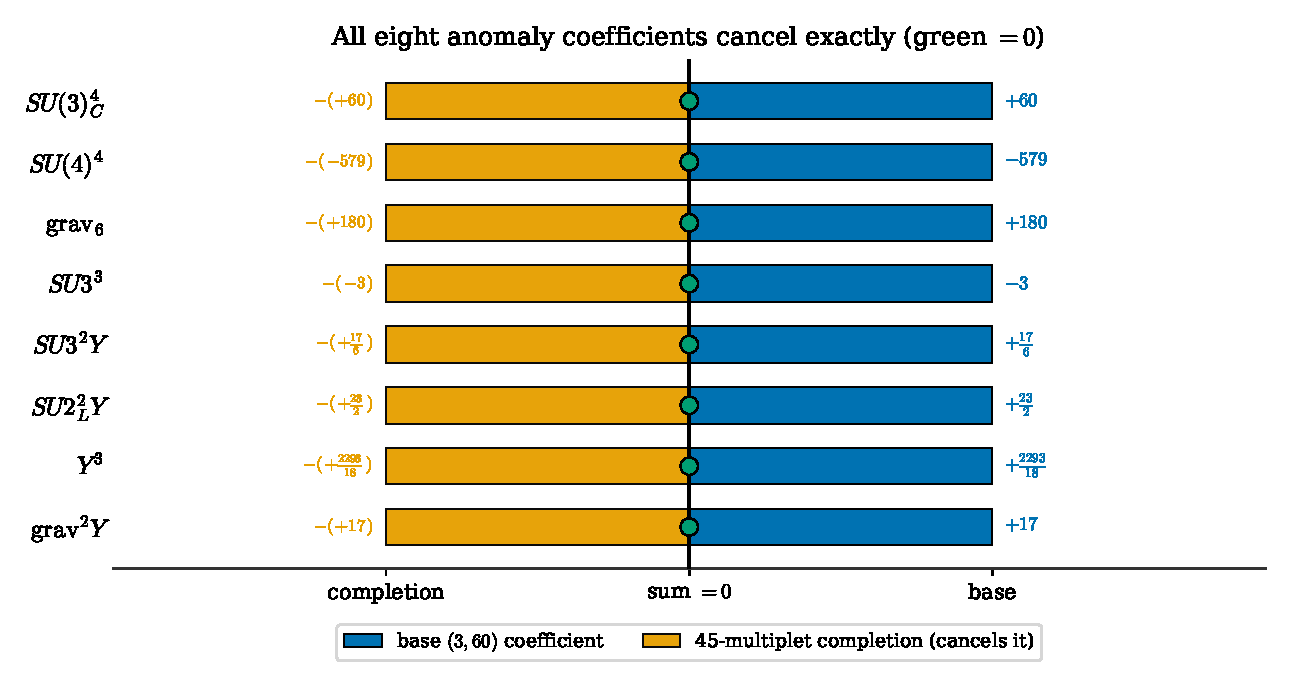
\includegraphics[width=0.82\linewidth]{fig_anomaly_cancel.pdf}
\caption{The eight bulk and four-dimensional zero-mode anomaly coefficients of the base
$(3,\mathbf{60})$ block (right, blue) and the exactly opposite contribution of the
$45$-multiplet completion (left, orange); each pair sums to zero (green). Coefficients
are exact rationals, recomputed independently.}
\label{fig:anomcancel}
\end{figure}

\begin{figure}[t]
\centering
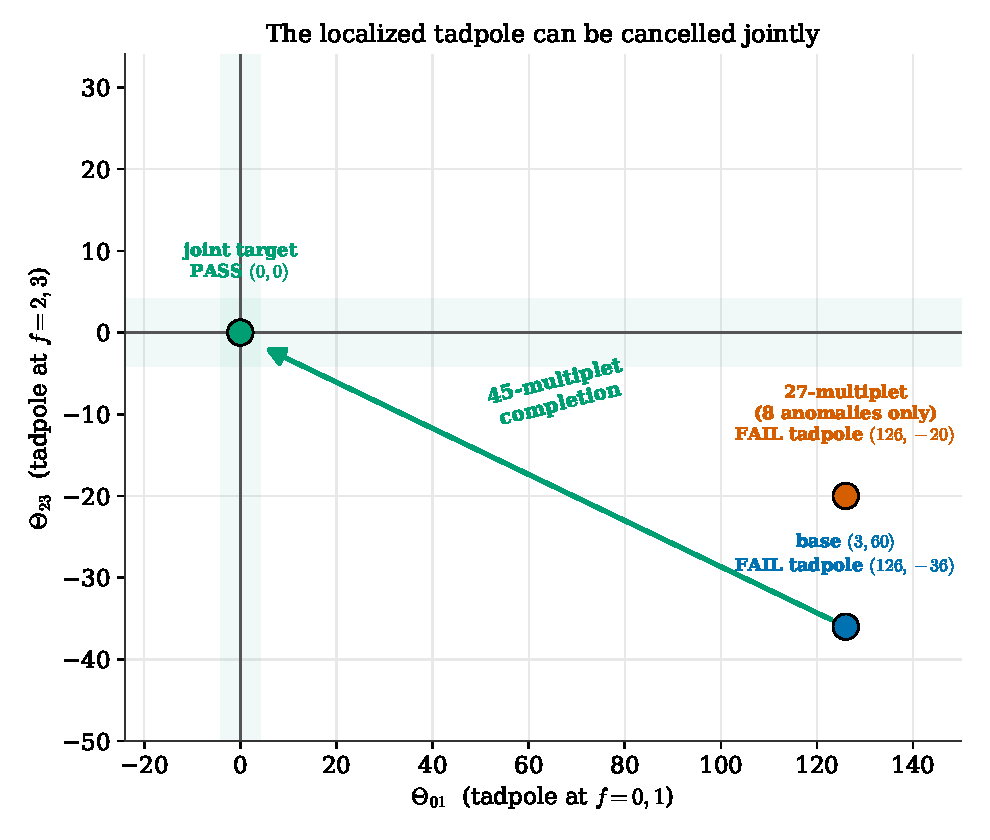
\includegraphics[width=0.80\linewidth]{fig_tadpole_journey.pdf}
\caption{The localized-tadpole plane $(\Theta_{01},\Theta_{23})$. The base block sits
at $\Theta_{\rm base}=(126,-36)$ and \emph{fails} the tadpole; the eight-anomaly
witness of $27$ multiplets moves only to $(126,-20)$ and still fails; the
$45$-multiplet completion (green arrow) brings the total to the origin. Anomaly freedom
alone does not cancel the tadpole --- but a joint completion does.}
\label{fig:tadmap}
\end{figure}

\begin{figure}[t]
\centering
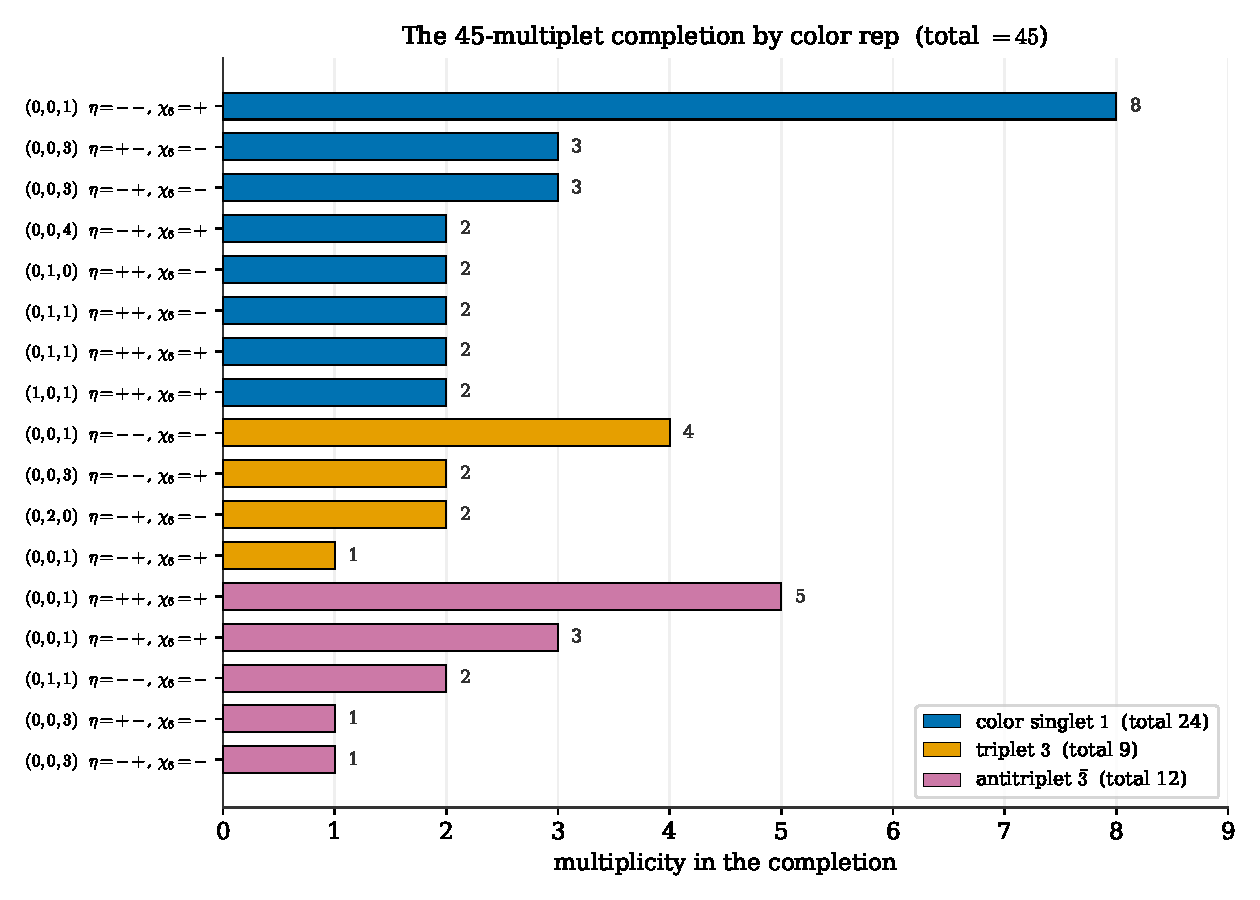
\includegraphics[width=0.86\linewidth]{fig_spectrum45.pdf}
\caption{The $45$-multiplet completion, grouped by color representation (Dynkin label,
intrinsic parity $\eta$, six-dimensional chirality $\chi_6$; multiplicities sum to
$45$). \textbf{Verified: eight anomalies $+$ localized tadpole $+$ local cubic
integrality; the mass gate ($\S\ref{sec:n7}$) pending.}}
\label{fig:witness45}
\end{figure}

\begin{table}[t]
\centering\small
\rowcolors{2}{softgrey}{white}
\begin{tabular}{clcccc}
\toprule
\rowcolor{hdrblue}
\textcolor{white}{\#} & \textcolor{white}{Dynkin $(a,b,c)$} & \textcolor{white}{color} &
\textcolor{white}{$\eta=(p_0,p_2)$} & \textcolor{white}{$\chi_6$} & \textcolor{white}{mult.}\\
\midrule
1  & $(0,0,1)$ & $\mathbf{1}$ & $(-,-)$ & $+$ & 8\\
2  & $(0,0,3)$ & $\mathbf{1}$ & $(+,-)$ & $-$ & 3\\
3  & $(0,0,3)$ & $\mathbf{1}$ & $(-,+)$ & $-$ & 3\\
4  & $(0,0,4)$ & $\mathbf{1}$ & $(-,+)$ & $+$ & 2\\
5  & $(0,1,0)$ & $\mathbf{1}$ & $(+,+)$ & $-$ & 2\\
6  & $(0,1,1)$ & $\mathbf{1}$ & $(+,+)$ & $-$ & 2\\
7  & $(0,1,1)$ & $\mathbf{1}$ & $(+,+)$ & $+$ & 2\\
8  & $(1,0,1)$ & $\mathbf{1}$ & $(+,+)$ & $+$ & 2\\
\rowcolor{white}\multicolumn{5}{r}{\textit{color singlets subtotal}} & \textit{24}\\
9  & $(0,0,1)$ & $\mathbf{3}$ & $(-,+)$ & $+$ & 1\\
10 & $(0,0,1)$ & $\mathbf{3}$ & $(-,-)$ & $-$ & 4\\
11 & $(0,0,3)$ & $\mathbf{3}$ & $(-,-)$ & $+$ & 2\\
12 & $(0,2,0)$ & $\mathbf{3}$ & $(-,+)$ & $-$ & 2\\
\rowcolor{white}\multicolumn{5}{r}{\textit{triplets subtotal}} & \textit{9}\\
13 & $(0,0,1)$ & $\bar{\mathbf{3}}$ & $(+,+)$ & $+$ & 5\\
14 & $(0,0,1)$ & $\bar{\mathbf{3}}$ & $(-,+)$ & $+$ & 3\\
15 & $(0,0,3)$ & $\bar{\mathbf{3}}$ & $(+,-)$ & $-$ & 1\\
16 & $(0,0,3)$ & $\bar{\mathbf{3}}$ & $(-,+)$ & $-$ & 1\\
17 & $(0,1,1)$ & $\bar{\mathbf{3}}$ & $(-,-)$ & $-$ & 2\\
\rowcolor{white}\multicolumn{5}{r}{\textit{antitriplets subtotal}} & \textit{12}\\
\midrule
\rowcolor{hdrblue}\multicolumn{5}{r}{\textcolor{white}{\textbf{total}}} & \textcolor{white}{\textbf{45}}\\
\bottomrule
\end{tabular}
\caption{The complete $45$-multiplet completion: all $17$ species by $SU(4)$ Dynkin label
$(a,b,c)$, color representation, intrinsic parity $\eta=(p_0,p_2)$, six-dimensional
chirality $\chi_6$, and multiplicity. This is the spectrum that cancels the eight anomaly
coefficients and the localized tadpole with integral local cubic residues
(\S\ref{sec:witness}); independently re-verified in exact rational arithmetic by
\texttt{r60\_verify\_joint.sage}.}
\label{tab:spectrum}
\end{table}

% ===================================================================
\section{From a witness to a guarantee: the tadpole never obstructs}\label{sec:existence}
Every model-builder knows the quiet doubt that trails a lucky find: was that a law, or
just this once? The $45$-multiplet spectrum of the previous section cancels the anomalies
and the tadpole together --- but one example is a coincidence until shown otherwise, and
the whole temper of this paper is to prefer a certificate to a coincidence. So we press
the sharper question the witness cannot answer on its own: is joint cancellation
\emph{inevitable}, or did $(3,\mathbf{60})$ simply get lucky? The answer, it turns out,
needs no further search --- only two elementary facts, because the anomalies and the
tadpole are both \emph{linear} functionals of the added multiplicities. Write $A$ for the
anomaly map (to $\mathbb{Q}^8$) and $\Theta$ for the localized-tadpole map (to
$\mathbb{Q}^2$) on the library of additions. Two questions then decide everything. First:
are the tadpole and the anomalies \emph{independent} dials, or is there a hidden
combination $\varphi\circ\Theta$ that stays fixed once the anomalies are cancelled --- a
conservation law that would pin the tadpole away from zero? Second: since one may only
\emph{add} matter, never subtract, can the additions that leave all eight anomalies
untouched still push the tadpole in \emph{every} direction? Both answers turn out
favorable, and exactly so.

Return now to the question left open in the introduction --- the one Scrucca, Serone,
Silvestrini and Wulzer posed in 2003. For two decades it stood dry: everyone agreed that a
realistic model needed an anomaly-free spectrum with a globally vanishing tadpole, everyone
knew the two constraints were independent, and yet the joint solution was treated as a
model-by-model hope --- something to stumble on, not something guaranteed. The two
questions above end that drought. The first, independence, was already their observation;
our part is to make it \emph{exact} --- a full-rank determinant certificate over the entire
library, not a remark in passing. The second question is the genuinely new one, and its
answer is the turn of the story: anomaly-neutral matter reaches \emph{every} tadpole value.
That single fact converts independence into a no-obstruction \emph{guarantee}, and settles
the twenty-two-year-old requirement --- not for one fortunate spectrum, but structurally,
for the whole class at once. It is our main structural result.

Why did the question stand for so long? Not for any want of effort --- the field circled
it for two decades --- but because it was being asked in the wrong language, and sought in
the wrong place. Model-building, by long habit, is a search: choose a fermion content, ask
whether the anomalies cancel \emph{and} the tadpole vanishes, and when they do not --- as,
almost always, they do not --- choose another and begin again. It is a treadmill, and
every failed step murmurs the same discouraging suggestion, that perhaps no step exists at
all; SSSW's closing note carries exactly that fatigue. And the roads the field \emph{did}
take led elsewhere. One tradition sought to \emph{forbid} the tadpole outright, by
arranging a symmetry under which it cannot arise --- the ``Higgs-gauge unification without
tadpoles'' of Biggio and Quir\'os~\cite{BiggioQ} --- a genuine escape, but one open only in
special configurations, and no help at all in cancelling a tadpole that is already there.
Another leaned on the oldest reflex for anomalies: add \emph{vector-like} matter, which
kills them for free. Yet the localized tadpole is blind to chirality, so a vector-like
pair \emph{doubles} it rather than relieving it --- the most familiar instrument in the
model-builder's hand is, here, exactly the wrong one. What the problem quietly asked for
was the opposite gesture: to add \emph{chiral} matter, each species anomalous on its own
yet summing to nothing, and enough of it to steer the tadpole home --- an unnatural thing
to attempt by hand, and an unnatural thing for a minimalist even to want. Independence, the
very thing SSSW had noticed, is moreover a false dawn here: knowing that the two dials turn separately does not
promise that both can be set to zero at once, because the model-builder is permitted only
to \emph{add} matter, never to take it away. The true object is therefore not a pair of
independent numbers but a \emph{cone} --- the set of tadpoles reachable by piling on
anomaly-neutral matter --- and a cone can be lopsided, opening toward one horizon and
walled off toward another. No one had drawn that cone. Two instincts kept it in the dark.
The first is a matter of vocabulary: the existence of \emph{some} completion, among all of
them, is a feasibility question --- of ranks, integer lattices, Farkas certificates ---
and those are the instruments of combinatorial optimization, a neighbouring country the
model-builder seldom visits, so the question was rarely even put in a form that could be
settled once and for all. The second is a matter of taste, and the more human of the two:
the completion that works is not lean but lavish --- forty-five multiplets poured in ---
and a discipline raised to admire economy does not go digging where the answer is heavy.
The solution sat in plain sight, in the one direction that aesthetics had told everyone
not to look. Trade the search for a feasibility test, set aside the reflex for minimality,
carry in the optimizer's tools --- and the twenty-two-year wall thins to nothing: a rank,
and a cone.

\begin{theorem}[Existence]\label{thm:existence}
Over the $SU(4)$ library (dimension $\le35$, all colors, parities and six-dimensional
chiralities), the combined map $(A,\Theta)$ has full rank $10=8+2$, and the image of
$\Theta$ on the anomaly-neutral non-negative cone $\{x\ge0:Ax=0\}$ is all of
$\mathbb{R}^2$. Consequently the localized tadpole imposes \emph{no} obstruction beyond
anomaly freedom: every anomaly-free completion of $(3,\mathbf{60})$ admits a
tadpole-compatible one. The $45$-multiplet spectrum is one realization, representative
rather than exceptional.
\end{theorem}

\noindent The proof is two exact certificates. \emph{Independence:} the stacked map
$[A;\Theta]$ has rank $10$ --- an explicit $10\times10$ integer minor has determinant
$3.6\times10^{20}\neq0$ --- so the two tadpole components are not any combination of the
eight anomaly coefficients and no invariant $\varphi\circ\Theta$ is conserved. (Were the
rank deficient, such a conserved combination would exist; the earlier anomaly-free
$27$-multiplet spectrum, which still carries tadpole $(126,-20)\neq0$, already shows the
tadpole is genuinely not fixed by the anomalies.) \emph{Reachability:} anomaly-neutral
non-negative additions realize each signed tadpole axis --- $\Theta=(288,0)$ by two
multiplets, $(0,48)$ by four, and their negatives likewise. Four directions that
positively span the plane put $0$ in the interior of the achievable cone, so whatever
residual tadpole an anomaly-free embedding carries, anomaly-neutral matter cancels it
(Figure~\ref{fig:cone}). Everything is exact rational linear algebra, and the four
witnesses together with their independence are re-checked in the Lean~4 kernel
(\texttt{R60JointExistence.lean}, depending only on \texttt{propext}). \hfill$\square$

\begin{figure}[t]
\centering
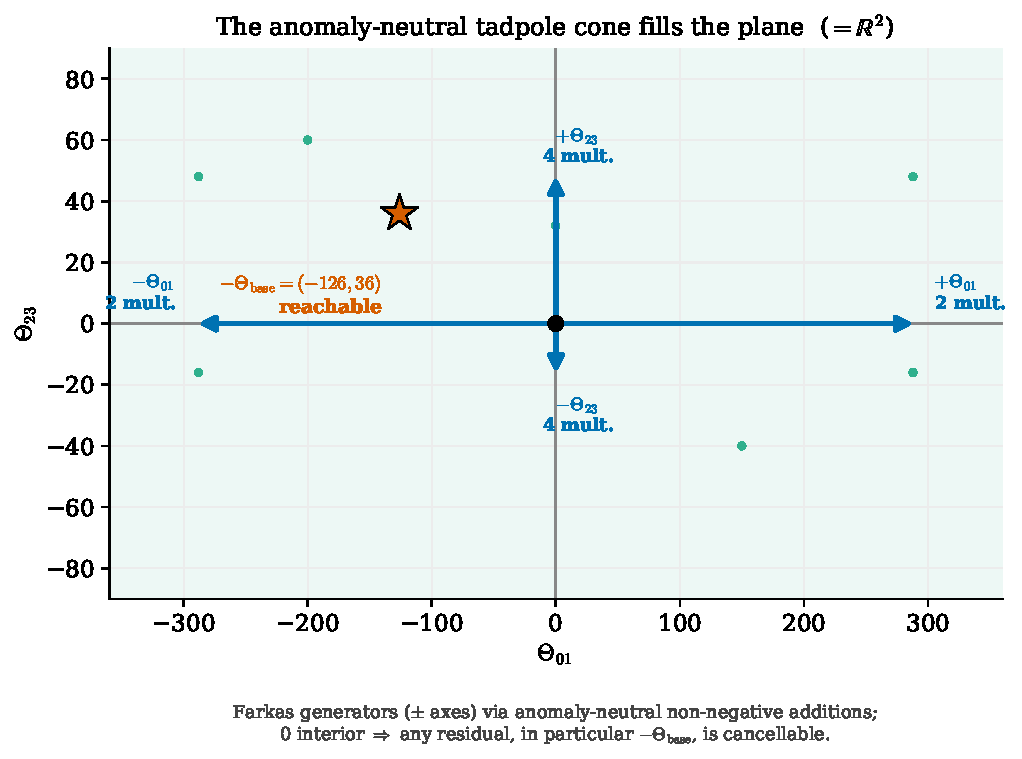
\includegraphics[width=0.70\linewidth]{fig_cone.pdf}
\caption{Theorem~\ref{thm:existence}, visually. Anomaly-neutral non-negative additions
realize both signs of each tadpole axis (blue arrows, labeled by the number of multiplets
--- the Farkas certificates), so the cone they generate is the whole plane $\mathbb{R}^2$
(shaded). The origin is interior; hence the base residual $-\Theta_{\rm base}=(-126,36)$
(star) --- and any other --- is cancellable by adding anomaly-neutral matter.}
\label{fig:cone}
\end{figure}

Behind the linear algebra is a picture worth keeping. The tadpole is a \emph{soft}
quantity --- a signed, parity-weighted sum whose sign flips with the intrinsic parity and
six-dimensional chirality of the matter one adds --- while the anomaly polynomials are
rigid. The fermion catalogue is thus rich enough to \emph{steer} the tadpole wherever one
likes, in any direction, without nudging a single anomaly coefficient. Read this way the
$45$-multiplet spectrum was never a needle in a haystack: the haystack is made of needles,
and we merely picked one up.

And the method outlives the example. The argument's form is model-independent: for
\emph{any} orbifold fermion library the same
\textbf{rank\,$+$\,cone} test decides whether a localized functional is an independent
obstruction (a conserved invariant, or a pointed cone --- an immediate no-go when the base
violates it) or is always absorbable. We release it as the ancillary tool
\texttt{ghu\_preflight.py}: given a fermion library (representations, colors, parities,
chiralities) and a base block, it returns the exact verdict --- \textsc{unobstructed},
\textsc{no-go} or \textsc{cone-obstructed} --- with its rank/Farkas certificate, the
physics model a single pluggable callback. Per model one obtains a decisive verdict; when
obstructed, the explicit conserved invariant $\varphi\circ\Theta$ (a candidate low-energy
signature); when unobstructed, a guarantee that an integer search terminates successfully
together with the constructive Farkas directions to \emph{build} a completion without a
solver; and, run over a family of embeddings, a classification of the landscape into
obstructed and unobstructed. It is thus an exact preflight before an expensive search ---
decision-complete on both sides --- and a way to hunt the genuinely obstructed models,
where anomaly freedom fails to imply tadpole freedom.

With that, the middle act of the story closes, and cleanly: the $(3,\mathbf{60})$ block is
\emph{consistent}, and provably so --- by a law, not an example. \emph{Established:}
tadpole cancellation is no obstruction beyond anomaly freedom; every anomaly-free
completion admits one. \emph{Left open:} the fully general integer statement over all
embeddings (a finite Hilbert-basis check --- the rational cone is already the whole plane).
What the block is not yet known to be is \emph{viable}; and for that the last and
strictest question of the journey remains.

% ===================================================================
\section{The boundary-mass filter and the physical verdict}\label{sec:n7}
A completion that is anomaly- and tadpole-consistent still carries exotic zero modes.
Boundary masses can pair them off, but the sharp question is whether they can do so
while leaving $Q$, $u_R$, $d_R$ massless. A localized Dirac mass at a fixed point pairs
a bulk zero mode with a brane Weyl fermion of conjugate local representation and opposite
four-dimensional chirality; whether \emph{all} exotics can be so lifted while every
target stays in the kernel is exactly a bipartite-matching (generic-rank) condition on
the allowed-mass graph. This is a finite, exact test --- it terminates with a definite
verdict rather than a timeout --- and we have validated the solver on known-answer
cases. Two structural facts sharpen it: the exotic left- and right-handed zero modes
carry mismatched $SU(2)_L$ representations, so brane partners are unavoidable; and the
multiplicity-two $Q_L$ means one must lift one degenerate doublet while protecting its
twin, a rank-deficiency that is possible but not automatic.

Running this gate against the full brane library at the two fixed-point classes, and
imposing the global $SU(2)$ parity that forbids an odd number of Weyl doublets (the
Witten anomaly~\cite{Witten82}), is the decisive physical step. We report
it as open: the verdict determines whether the $(3,\mathbf{60})$ completion is viable
--- a realistic quark sector of the AHMN two-Higgs-doublet model --- or a no-go, in
which case the obstruction carries a concrete low-energy signature (unavoidable light
exotics or a vector-like partner of a Standard-Model quark). Either outcome is a result
of the exact hierarchy; neither is claimed here.

% ===================================================================
\section{Low-energy signatures of the two verdicts}\label{sec:signatures}
Grant the exact hierarchy its two possible answers --- what would each look like in an
experiment? The value of pinning the consistency question down is that the two outcomes
are not phenomenologically interchangeable: each maps to a distinct, and in principle
falsifiable, low-energy signature. One robust prediction survives either way. Because
the underlying AHMN construction delivers \emph{two} Higgs doublets as Wilson-line zero
modes~\cite{AHMN}, the scalar sector is that of a two-Higgs-doublet model, with the
attendant extra states $H$, $A$, $H^\pm$ and the flavor-alignment questions such models
carry~\cite{2HDM}; in gauge--Higgs unification their potential is radiative and finite,
so the doublet masses and mixings are tied to the compactification dynamics rather than
free~\cite{Hosotani}. Our analysis does not compute those masses, but it fixes the
setting in which they live.

If the boundary-mass filter \emph{passes} --- every exotic lifted at the
compactification scale $1/R$ while $Q,u_R,d_R$ stay massless --- the light theory is the
Standard Model plus that second doublet, and the distinctive high-scale imprint is a
tower of Kaluza--Klein excitations of the gauge and matter fields at $1/R$, the generic
fingerprint of the extra dimensions. If instead the filter returns a \emph{no-go}, the
obstruction is not abstract: the rank-deficiency of the matching leaves a physical
remnant. Two shapes are possible. Either an exotic zero mode cannot be paired at all and
survives as an unavoidable light state --- a colored or weak-charged particle near the
electroweak-to-TeV window, the sharpest possible falsifier --- or the only way to lift
the exotic doublet is to pair it with a partner that also marries a Standard-Model quark,
leaving a \emph{vector-like quark}: a non-chiral partner of $Q$, $u_R$ or $d_R$ that
mixes with the light generations and is searched for directly at colliders through
single and pair production~\cite{VLQ}. The multiplicity-two $Q_L$ isolated in
\S\ref{sec:hypercharge} is exactly what makes this second option natural --- two doublets
of identical charges, one of which must be given a vector-like mass --- so a vector-like
$Q$-partner is the specific signature a no-go here would carry.

How heavy, and how would one tell them apart? Gauge--Higgs unification ties the
compactification scale $1/R$ to the radiatively generated Higgs mass; reproducing
$m_h=125$~GeV with a top-driven Coleman--Weinberg potential typically pushes $1/R$ into
the multi-TeV range, so the Kaluza--Klein tower and the heavier scalars of the
two-doublet sector would sit there, at or beyond current collider reach. A vector-like
quark need not, however, live at $1/R$: if it arises from a boundary-mass
rank-deficiency, its mass is a brane parameter and could be considerably lighter, within
the reach of the LHC and its high-luminosity phase. Such a state would announce itself
in the established vector-like-quark channels~\cite{VLQ} --- pair production followed by
decays to $Wq$, $Zq$ or $hq$, or single production through its mixing with the light
generations --- and the multiplicity-two $Q_L$ points specifically to a partner in the
$(t,b)$ doublet sector. The other no-go branch, an exotic that cannot be paired at all,
would instead surface as a stable or long-lived colored or weak-charged state near the
electroweak scale, a sharper and more immediately falsifiable signal. The distinction is
therefore not academic: one verdict places the new physics at $1/R$ far above, the other
a vector-like quark possibly already in range. None of these masses is computed here ---
they are downstream of the mass filter and the compactification data --- but the
\emph{classes} of signal are fixed by the structure established above.

\emph{Established:} whichever way the verdict falls, the framework robustly predicts a
second Higgs doublet, and the two verdicts separate cleanly into a Kaluza--Klein/2HDM
spectrum on the one hand and a light-exotic or vector-like-quark signature on the other.
\emph{Left open:} which of these the model realizes, and the scale $1/R$ that sets the
masses --- neither computed here, both downstream of the mass filter.

% ===================================================================
\section{Consistency, viability, and what an exact answer buys us}\label{sec:reflection}
What does this concrete exercise teach about the gap between a consistent theory and a
viable one? The case sharpens a distinction easy to blur. \emph{Consistency} --- anomaly
freedom, tadpole cancellation --- is a statement about the ultraviolet; \emph{viability}
--- a light spectrum that is the Standard Model and nothing else --- is a statement about
the infrared. Gauge--Higgs unification makes the seam visible: the Higgs is a Wilson
line, so the same orbifold data that fix the anomalies also shape the Higgs potential,
yet the anomaly obstruction is topological and blind to the Higgs vacuum, while the mass
of the exotics is a spectral, infrared question. A model can be perfectly consistent and
still fail to be viable, and only an infrared filter --- here the boundary-mass matching
--- decides.

There is a reflection about the Higgs itself, and why it stays so hard to pin down. In
gauge--Higgs unification the same internal components $A_5,A_6$ are simultaneously gauge
field and Higgs; which of the two the theory shows depends on the vacuum it sits in, so
the Higgs has no fixed identity independent of the Wilson line it rides. That elusiveness
is not a nuisance but the source of its good behavior --- an object with no local
definition admits no local mass counterterm --- and it is exactly what the localized
tadpole threatens to spoil, by feeding a fixed-point term straight into a mass the
mechanism was built to protect. Read this way the entire consistency hierarchy is a set
of conditions for keeping the Higgs elusive: anomaly freedom and tadpole cancellation are
the price of a scalar that is protected precisely because it is never quite a scalar. The
completion we exhibit pays that price at the orbifold level; whether the infrared then
delivers a Standard-Model Higgs and nothing else is the question the mass filter holds.

There is a methodological reflection too. Where, when the arithmetic is machine-checked,
does the last freedom to be wrong live? Not in the numbers --- in the sentence that names
them. When each link of the argument is a
machine-verifiable certificate, the failure mode of model-building shifts: the danger is
no longer an arithmetic slip but a \emph{misinterpretation} --- a true number attached to
a false sentence. Making the pipeline exact does not remove that danger, but it isolates
it, and lets a wrong turn be caught by the ground truth rather than by taste. Several
plausible intermediate claims in this very study were refuted that way before entering
the paper --- a factor-of-two normalization in the hypercharge, and a proposed
vector-like correction of the tadpole that the integer lattice ruled out. In that sense the contribution is as much about \emph{how} such
questions can be settled as about the particular answer for $(3,\mathbf{60})$.

% ===================================================================
\section{Reflections on the problem, and the directions it opens}\label{sec:outlook}
Step back from $(3,\mathbf{60})$ for a moment. In orbifold model-building the local data ---
localized anomalies, tadpoles, boundary masses --- have long been treated as a checklist of
separate hazards, each cleared by hand. What the exact view adds is that these conditions
have an \emph{algebra}: some are rigid and mutually constraining (the anomaly polynomials),
others soft and freely steerable (the tadpole), and whether a given local condition is a
genuine obstruction is not a matter of luck to be discovered by search but a structural fact
to be computed once. A landscape of case-by-case checks becomes a small number of decidable
questions. Three threads follow naturally, and we flag them as proposals rather than
promises.

\emph{First, close the concrete case.} The one verdict still open for $(3,\mathbf{60})$ is
viability: assembling the brane library at the two fixed-point classes and running the
boundary-mass matching of \S\ref{sec:n7} is a finite, exact test with a definite yes/no ---
either a realistic quark sector of the AHMN two-doublet model, or a certified no-go with a
concrete signature (a light exotic or a vector-like partner).

\emph{Second, harden and machine-check the structure.} The Existence theorem is proved over
$\mathbb{Q}$ with the integer statement settled for $(3,\mathbf{60})$ by the witness; the
fully general integer form is a finite Hilbert-basis step. Both it and the rank/Farkas
certificates are of a shape a proof assistant handles well, extending the localized-anomaly
Lean fragment to a verified \emph{structural} result --- a rare thing for a model-building
theorem.

\emph{Third, and most invitingly, sweep the landscape for obstructions.} The same
\textbf{rank\,$+$\,cone} test --- packaged as \texttt{ghu\_preflight.py} --- applies to any
orbifold group and matter (\,$SU(5)$, $SU(6)$, $E_6$, other representations\,) and to other
fixed-point data (localized Fayet--Iliopoulos terms, further local functionals). The
valuable target is not to confirm more unobstructed cases but to \emph{hunt the obstructed
ones}: embeddings where anomaly freedom demonstrably fails to force tadpole freedom. Each
such case carries a conserved invariant $\varphi\circ\Theta$ that is a concrete low-energy
signature --- a principled search for genuine no-go models, rather than one construction at a
time. In the larger picture this is a small instance of a program worth pursuing wherever a
model-building result currently reads ``we found one'': to ask whether the find was a law,
and to turn the computational witness into a structural theorem. The companion
Part~II~\cite{PartII} carries out exactly this program for the minimality found above,
turning the scanned fact that $(3,\mathbf{60})$ is the smallest admissible representation
into an exact classification of \emph{which} $SU(4)$ representations contain the
Standard-Model quark cell.

% ===================================================================
\section{Methodology and reproducibility}\label{sec:method}
Every claim above is a finite exact computation. Anomaly and tadpole coefficients are
exact rational sums over $SU(4)$ weights (SageMath); the coupled feasibility is studied
with exact branch-and-bound (PPL), OR-Tools CP-SAT, and layered lattice certificates
(Smith normal form), with the $45$-multiplet witness re-verified in exact rationals; the
boundary-mass gate is exact bipartite matching; and the localized-cubic fragment is
certified axiom-free in Lean~4. We are explicit about what is \emph{not} established: the
general bounded search is \texttt{UNKNOWN}, and a Hilbert-basis (Normaliz) certificate
was not produced at this dimension. The ancillary material contains the scripts, the
full $45$-multiplet spectrum, the constraint table with each condition's status and
scope, and the Lean source, so that every number here can be regenerated. The exact
computations were carried out and cross-checked by two independent agents working
against this common ground truth; that working method, rather than any single number,
is what most reduced the interpretation errors a model-building analysis is prone to.

Table~\ref{tab:artifacts} lists the machine-checkable artifacts released with this
paper; each entry regenerates a specific claim above.

\begin{table}[h]
\centering
\footnotesize
\rowcolors{2}{softgrey}{white}
\begin{tabular}{lll}
\toprule
\rowcolor{hdrblue}
\textcolor{white}{Artifact} & \textcolor{white}{Certifies} & \textcolor{white}{Tool}\\
\midrule
\texttt{R60LocalizedAnomaly.lean} & localized cubic residues, $\dim=60$, Wilson dependence & Lean~4 (axiom-free)\\
\texttt{R60JointExistence.lean}   & the Existence theorem's cone/independence certificate & Lean~4 (only \texttt{propext})\\
\texttt{r60\_sm\_embedding.sage}   & hypercharge $Y=(-7q_8+4q_{15})/18$; SM charges & SageMath (exact)\\
\texttt{r60\_anomalies.sage}       & eight bulk/zero-mode coefficients of $(3,\mathbf{60})$ & SageMath (exact)\\
\texttt{r60\_tadpole.sage}         & localized tadpole $\Theta_{\rm base}=(126,-36)$ & SageMath (exact)\\
\texttt{r60\_cpsat.sage}           & the $45$-multiplet joint completion search & OR-Tools CP-SAT\\
\texttt{r60\_verify\_joint.sage}   & independent re-check of the $45$-multiplet witness & SageMath (exact)\\
\texttt{r60\_n7\_matching.sage}    & boundary-mass bipartite gate (validated cases) & OR-Tools / exact\\
\texttt{structural\_theorem.sage} & $\operatorname{rank}[A;\Theta]=10$ and the tadpole cone (Thm~\ref{thm:existence}) & SageMath (exact)\\
\texttt{ghu\_preflight.py}        & reusable rank$+$cone obstruction oracle (any model) & SageMath (exact)\\
\texttt{make\_paper\_graphics.py}  & Figures~\ref{fig:anomcancel}--\ref{fig:witness45} from the verified data & Matplotlib\\
\bottomrule
\end{tabular}
\caption{Reproducibility manifest. Each artifact regenerates one claim in the paper; the
Lean file is checked by the kernel with no axioms beyond Lean's own and no \texttt{sorry}.
Released with the ancillary material.}
\label{tab:artifacts}
\end{table}

% ===================================================================
\section{Conclusion}\label{sec:conclusion}
The main lesson is concrete, and it closes a question older than the model at hand.
Anomaly freedom and localized-tadpole cancellation --- named \emph{independent} constraints
by Scrucca, Serone, Silvestrini and Wulzer in 2003, who left the construction of an
anomaly-free spectrum with a globally vanishing tadpole as an open problem --- are here not
merely compatible: the tadpole is proved to \emph{never} obstruct an anomaly-free
completion, so that after two decades their requirement is met not by luck but as a
structural guarantee, exact and machine-checked. The $(3,\mathbf{60})$ block, which a scan
shows to be the minimal representation able to host the quarks at all, realizes it
explicitly --- a $45$-multiplet completion cancelling all eight anomaly coefficients and
the localized tadpole \emph{together}, with integral local cubic residues and two
Lean-checked certificates. What remains is the sharpest question of all --- whether that
consistent spectrum is also physically viable, its exotics lifted and only the Standard
Model left light --- and it is the boundary-mass filter, itself an exact and finite test,
that will decide it. Consistency, here, has been settled with certificates; viability is
the next certificate to earn.

\appendix
% ===================================================================
\section{Group-theoretic conventions and the exact indices}\label{app:conventions}
So that every number above can be regenerated, we fix here the conventions the Lean and
Sage artifacts encode. An $SU(4)$ weight is written by its Young entries
$n_1\ge n_2\ge n_3\ge n_4$; the internal charges used throughout are
\begin{equation}
q_8=n_1+n_2-2n_3,\qquad q_{15}=n_1+n_2+n_3-3n_4,\qquad q_P=n_1+n_2-n_3-n_4,
\end{equation}
and the two orbifold parities of a weight are $p_0=(-1)^{n_4}$, $p_2=(-1)^{n_3+n_4}$.
The hypercharge \eqref{eq:Y}, $Y=(-7q_8+4q_{15})/18$, is the unique internal combination
assigning $Q_L,u_R,d_R$ their physical charges $1/6,2/3,-1/3$ (Table~\ref{tab:smcontent})
and preserving $\sin^2\theta_W=\tfrac14$ at tree level; the four $Y$-dependent anomaly
coefficients are quoted in this same normalization.

The four-dimensional zero-mode anomalies use the Dynkin index of the $SU(2)_L$ spin
content, $T_2(d)=\tfrac1{12}d(d^2-1)$ for an irrep of dimension $d$, weighted by the
color dimension and the six-dimensional chirality sign; the pure cubic $SU(3)^3$ uses
the fundamental cubic normalization. The six-dimensional coefficients use the quartic
index $A_4$ of the $SU(4)$ irrep (the coefficient of the primitive $\Tr_4 F^4$ after
subtracting the reducible $(\Tr F^2)^2$ part) and the representation dimension. For the
$SU(3)$ color factor there is \emph{no} primitive quartic Casimir, so
$\Tr_3 F_C^4=\tfrac12(\Tr_3 F_C^2)^2$ and the ``$SU(3)_C^4$'' entry is reducible; this is
the origin of the rank-two quadratic form of \S\ref{sec:bulkanom}. The localized cubic
residues at $f=0,1$ carry the fixed-point normalizations $\tfrac14$ (color) and
$-\tfrac18$ ($SU(3)_{123}$), and the tadpole components are
$\Theta_{01}\propto\sum \eta_0\,p_0\,q_{15}$ and $\Theta_{23}\propto\sum \eta_2\,p_2\,q_P$
over the weights, times the color dimension.

Under $SU(3)_C\times[SU(3)_{123}\times U(1)_{15}]$ the block $(3,\mathbf{60})$ with
$\eta=(+,+)$ decomposes into the electroweak zero modes of Table~\ref{tab:smcontent}
plus the exotics; the $45$-multiplet completion is listed by
$(\text{Dynkin},\text{color},\eta,\chi_6)$ with multiplicities in full in
Table~\ref{tab:spectrum} and in the ancillary \texttt{r60\_verify\_joint.sage}. All indices in this
appendix are recomputed exactly (no floating point) by that script and by
\texttt{R60LocalizedAnomaly.lean}.

\begin{thebibliography}{99}
\bibitem{PartII} C.~Mar\'in, \emph{Three Gates to a Quark Generation: An Exact Criterion for
Which $SU(4)$ Representations Contain the Standard Model} (Part~II), Zenodo (2026),
DOI:\,10.5281/zenodo.21432627.
% All arXiv/journal entries verified, 2026-07-18.
\bibitem{Manton} N.S.~Manton, \emph{A New Six-Dimensional Approach to the
Weinberg-Salam Model}, Nucl.\ Phys.\ B\textbf{158} (1979) 141.
\bibitem{Fairlie} D.B.~Fairlie, \emph{Higgs' fields and the determination of the
Weinberg angle}, Phys.\ Lett.\ B\textbf{82} (1979) 97.
\bibitem{Hosotani} Y.~Hosotani, \emph{Dynamical mass generation by compact extra
dimensions}, Phys.\ Lett.\ B\textbf{126} (1983) 309; Ann.\ Phys.\ \textbf{190} (1989) 233.
\bibitem{ColemanWeinberg} S.~Coleman, E.~Weinberg, \emph{Radiative Corrections as the
Origin of Spontaneous Symmetry Breaking}, Phys.\ Rev.\ D\textbf{7} (1973) 1888.
\bibitem{GreenSchwarz} M.B.~Green, J.H.~Schwarz, \emph{Anomaly Cancellation in
Supersymmetric $D=10$ Gauge Theory and Superstring Theory}, Phys.\ Lett.\ B\textbf{149}
(1984) 117.
\bibitem{Sagnotti} A.~Sagnotti, \emph{A note on the Green-Schwarz mechanism in
open-string theories}, Phys.\ Lett.\ B\textbf{294} (1992) 196, hep-th/9210127.
\bibitem{CallanHarvey} C.G.~Callan, J.A.~Harvey, \emph{Anomalies and Fermion Zero Modes
on Strings and Domain Walls}, Nucl.\ Phys.\ B\textbf{250} (1985) 427.
\bibitem{Witten82} E.~Witten, \emph{An $SU(2)$ Anomaly}, Phys.\ Lett.\ B\textbf{117}
(1982) 324.
\bibitem{KawamuraGUT} Y.~Kawamura, \emph{Triplet-doublet splitting, proton stability
and an extra dimension}, Prog.\ Theor.\ Phys.\ \textbf{105} (2001) 999, hep-ph/0103125.
\bibitem{ACG} N.~Arkani-Hamed, A.G.~Cohen, H.~Georgi, \emph{Anomalies on Orbifolds},
Phys.\ Lett.\ B\textbf{516} (2001) 395, hep-th/0103135.
\bibitem{GdVQ} G.~von Gersdorff, M.~Quir\'os, \emph{Localized anomalies in orbifold
gauge theories}, hep-th/0305024.
\bibitem{GdV6D} G.~von Gersdorff, \emph{Anomalies on Six Dimensional Orbifolds},
hep-th/0612212.
\bibitem{BiggioQ} C.~Biggio, M.~Quir\'os, \emph{Higgs-gauge unification without
tadpoles}, hep-ph/0407348.
\bibitem{SSSW} C.A.~Scrucca, M.~Serone, L.~Silvestrini, A.~Wulzer,
\emph{Gauge-Higgs Unification in Orbifold Models}, hep-th/0312267.
\bibitem{Kawamura} J.~Goto, Y.~Kawamura, T.~Miura, \emph{Orbifold Family Unification
on Six Dimensions}, arXiv:1307.2631.
\bibitem{aGUT} G.~Cacciapaglia, \emph{Systematic classification of aGUT models in five
dimensions: the $SU(N)$ kinship}, arXiv:2309.10098.
\bibitem{SU6GHGUT} A.~Angelescu, A.~Bally, F.~Goertz, S.~Weber, \emph{$SU(6)$
Gauge-Higgs Grand Unification: Minimal Viable Models and Flavor}, arXiv:2208.13782.
\bibitem{AHMN} K.~Akamatsu, T.~Hirose, N.~Maru, A.~Nago, \emph{Two Higgs Doublet Model
from Six Dimensional Gauge Theory}, arXiv:2603.05857.
\bibitem{2HDM} G.C.~Branco, P.M.~Ferreira, L.~Lavoura, M.N.~Rebelo, M.~Sher, J.P.~Silva,
\emph{Theory and phenomenology of two-Higgs-doublet models}, Phys.\ Rept.\ \textbf{516}
(2012) 1, arXiv:1106.0034.
\bibitem{VLQ} J.A.~Aguilar-Saavedra, R.~Benbrik, S.~Heinemeyer, M.~P\'erez-Victoria,
\emph{Handbook of vectorlike quarks: Mixing and single production}, Phys.\ Rev.\
D\textbf{88} (2013) 094010, arXiv:1306.0572.
\end{thebibliography}

\end{document}
